\chapter{Entwurf}
\label{ch:3}

\section{Grobentwurf: Subsysteme}
\label{sec:3.1}
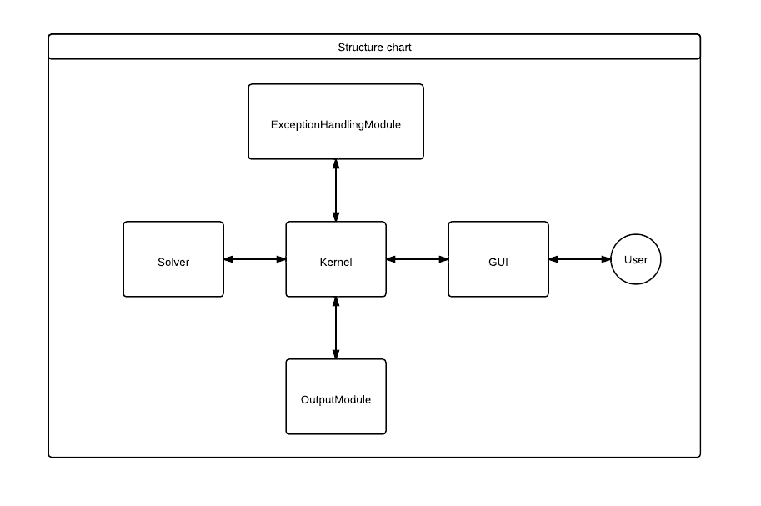
\includegraphics[width=4in,keepaspectratio=true]{figures/StructureDiagGyroSim.png}

\section{Detailentwurf: Klassen}
\label{sec:3.2}
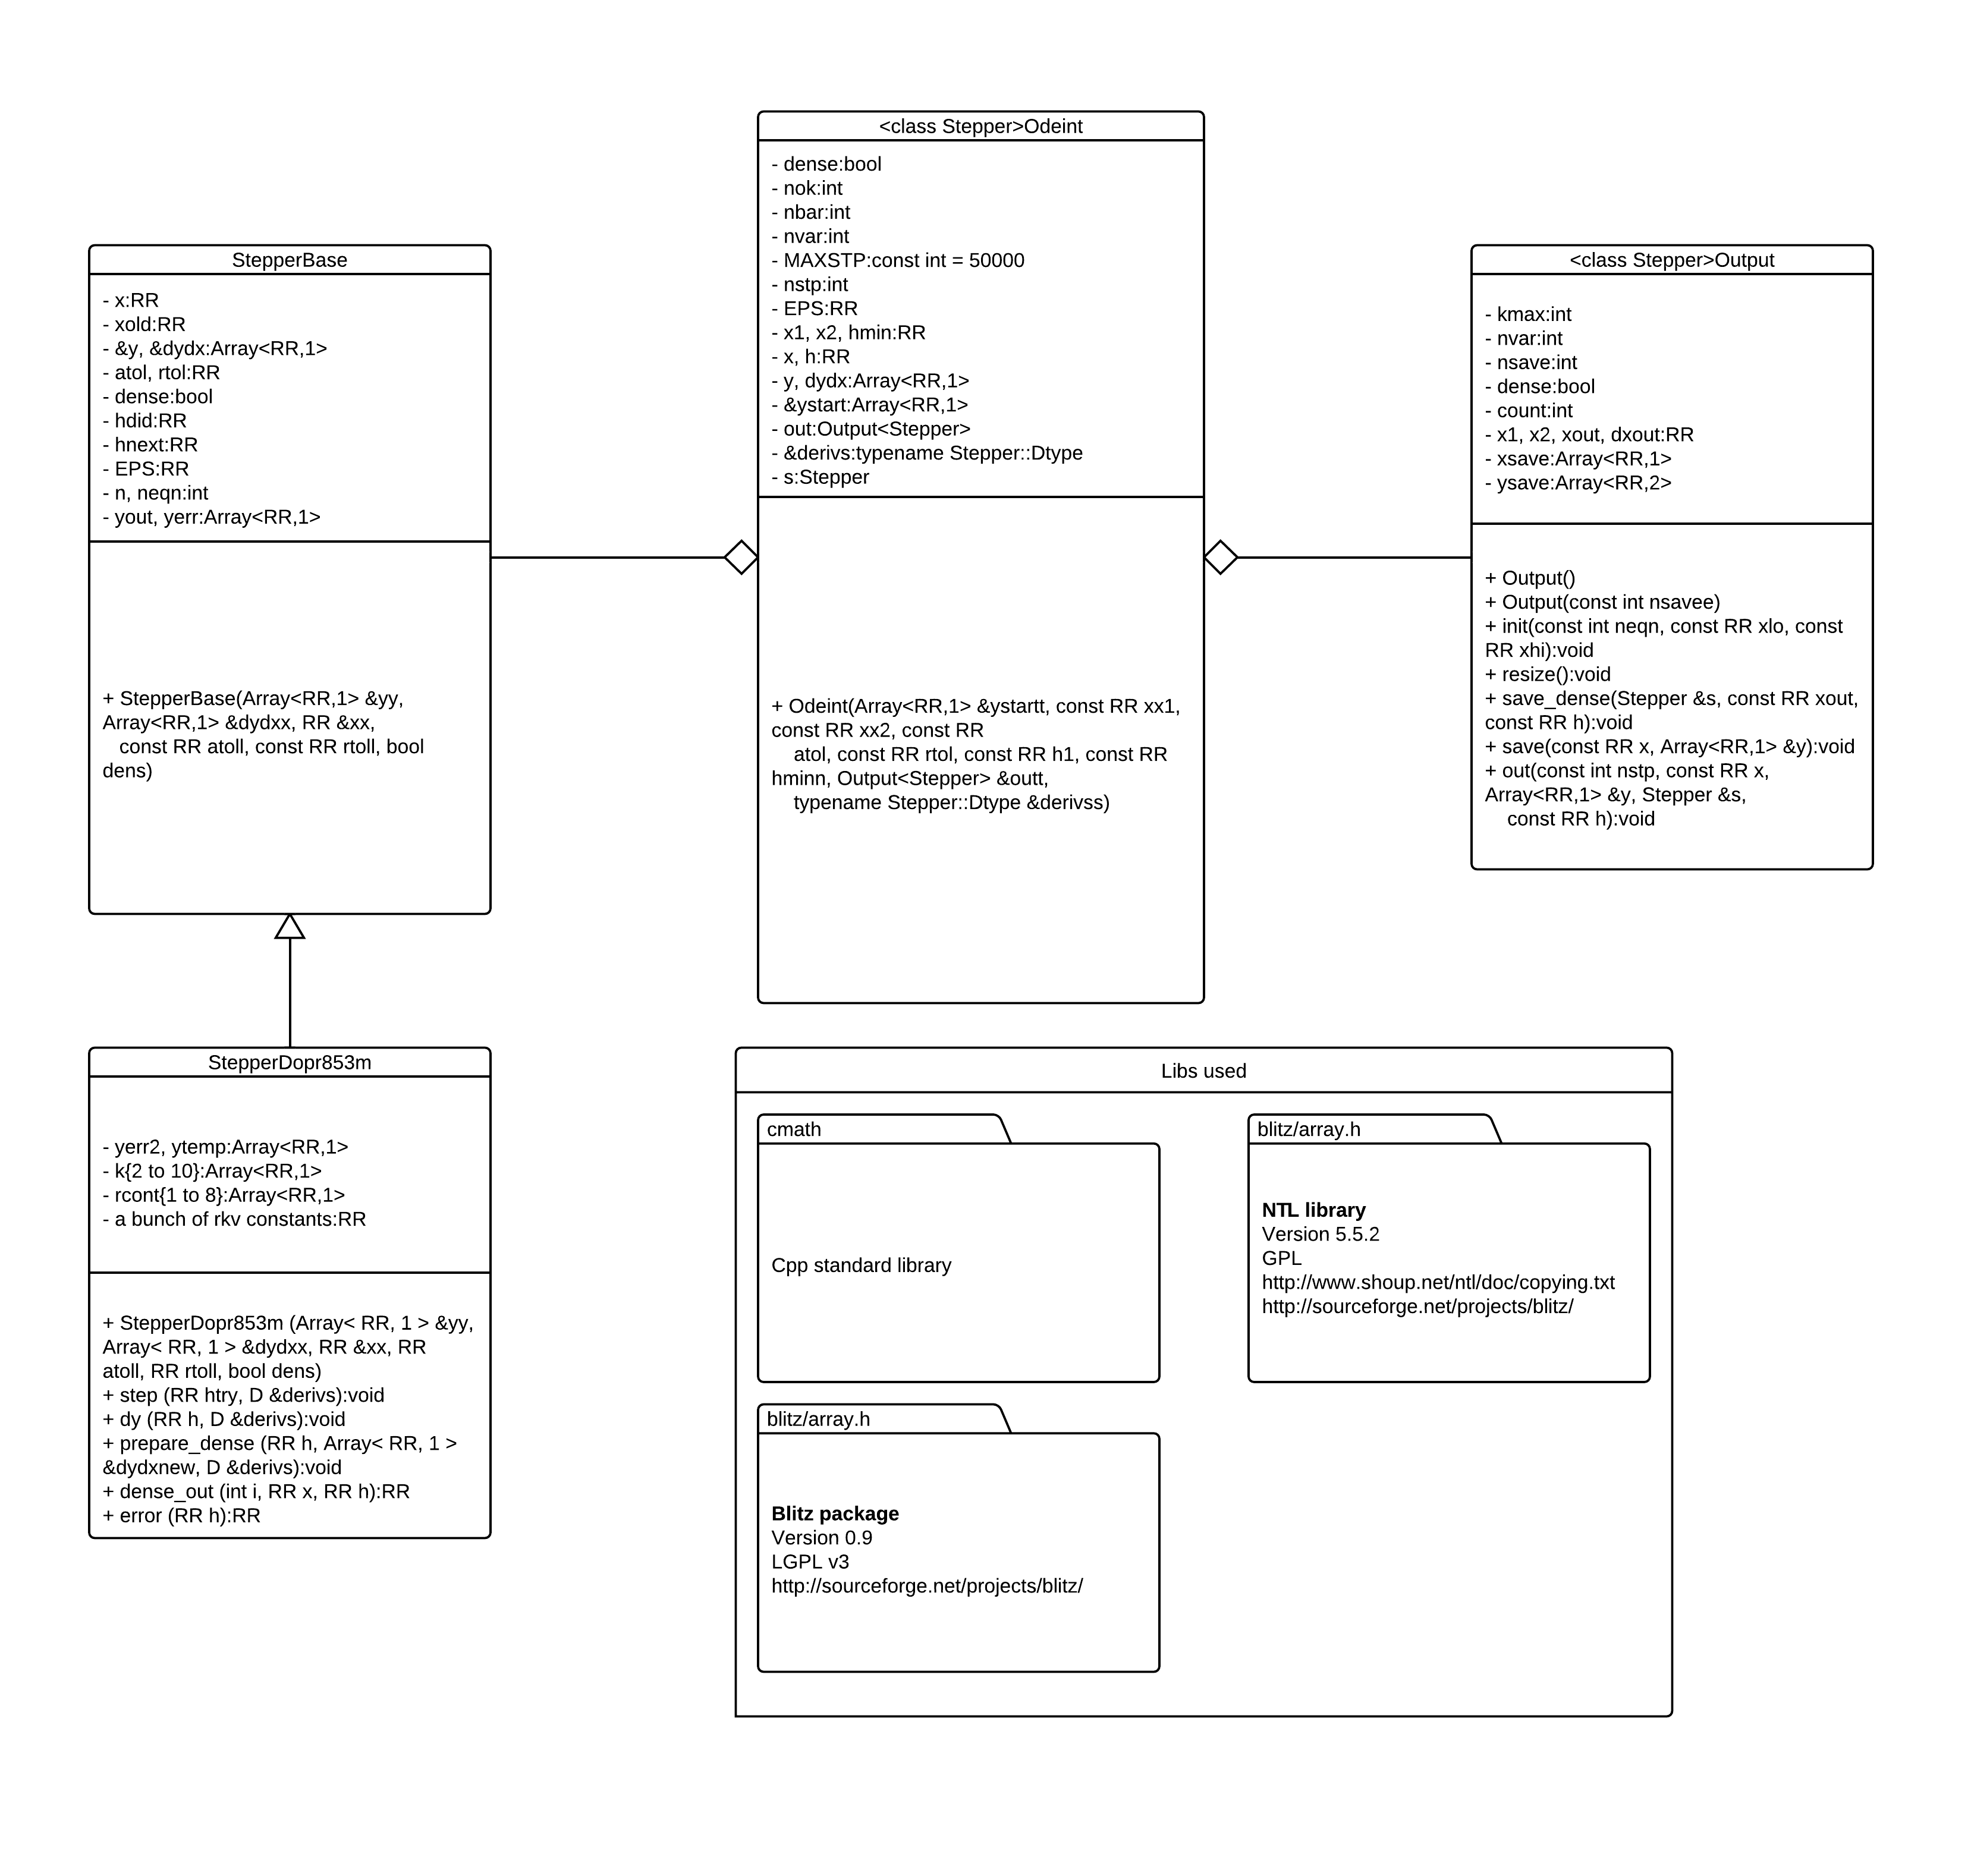
\includegraphics[width=4in,keepaspectratio=true]{figures/Odeint.png}

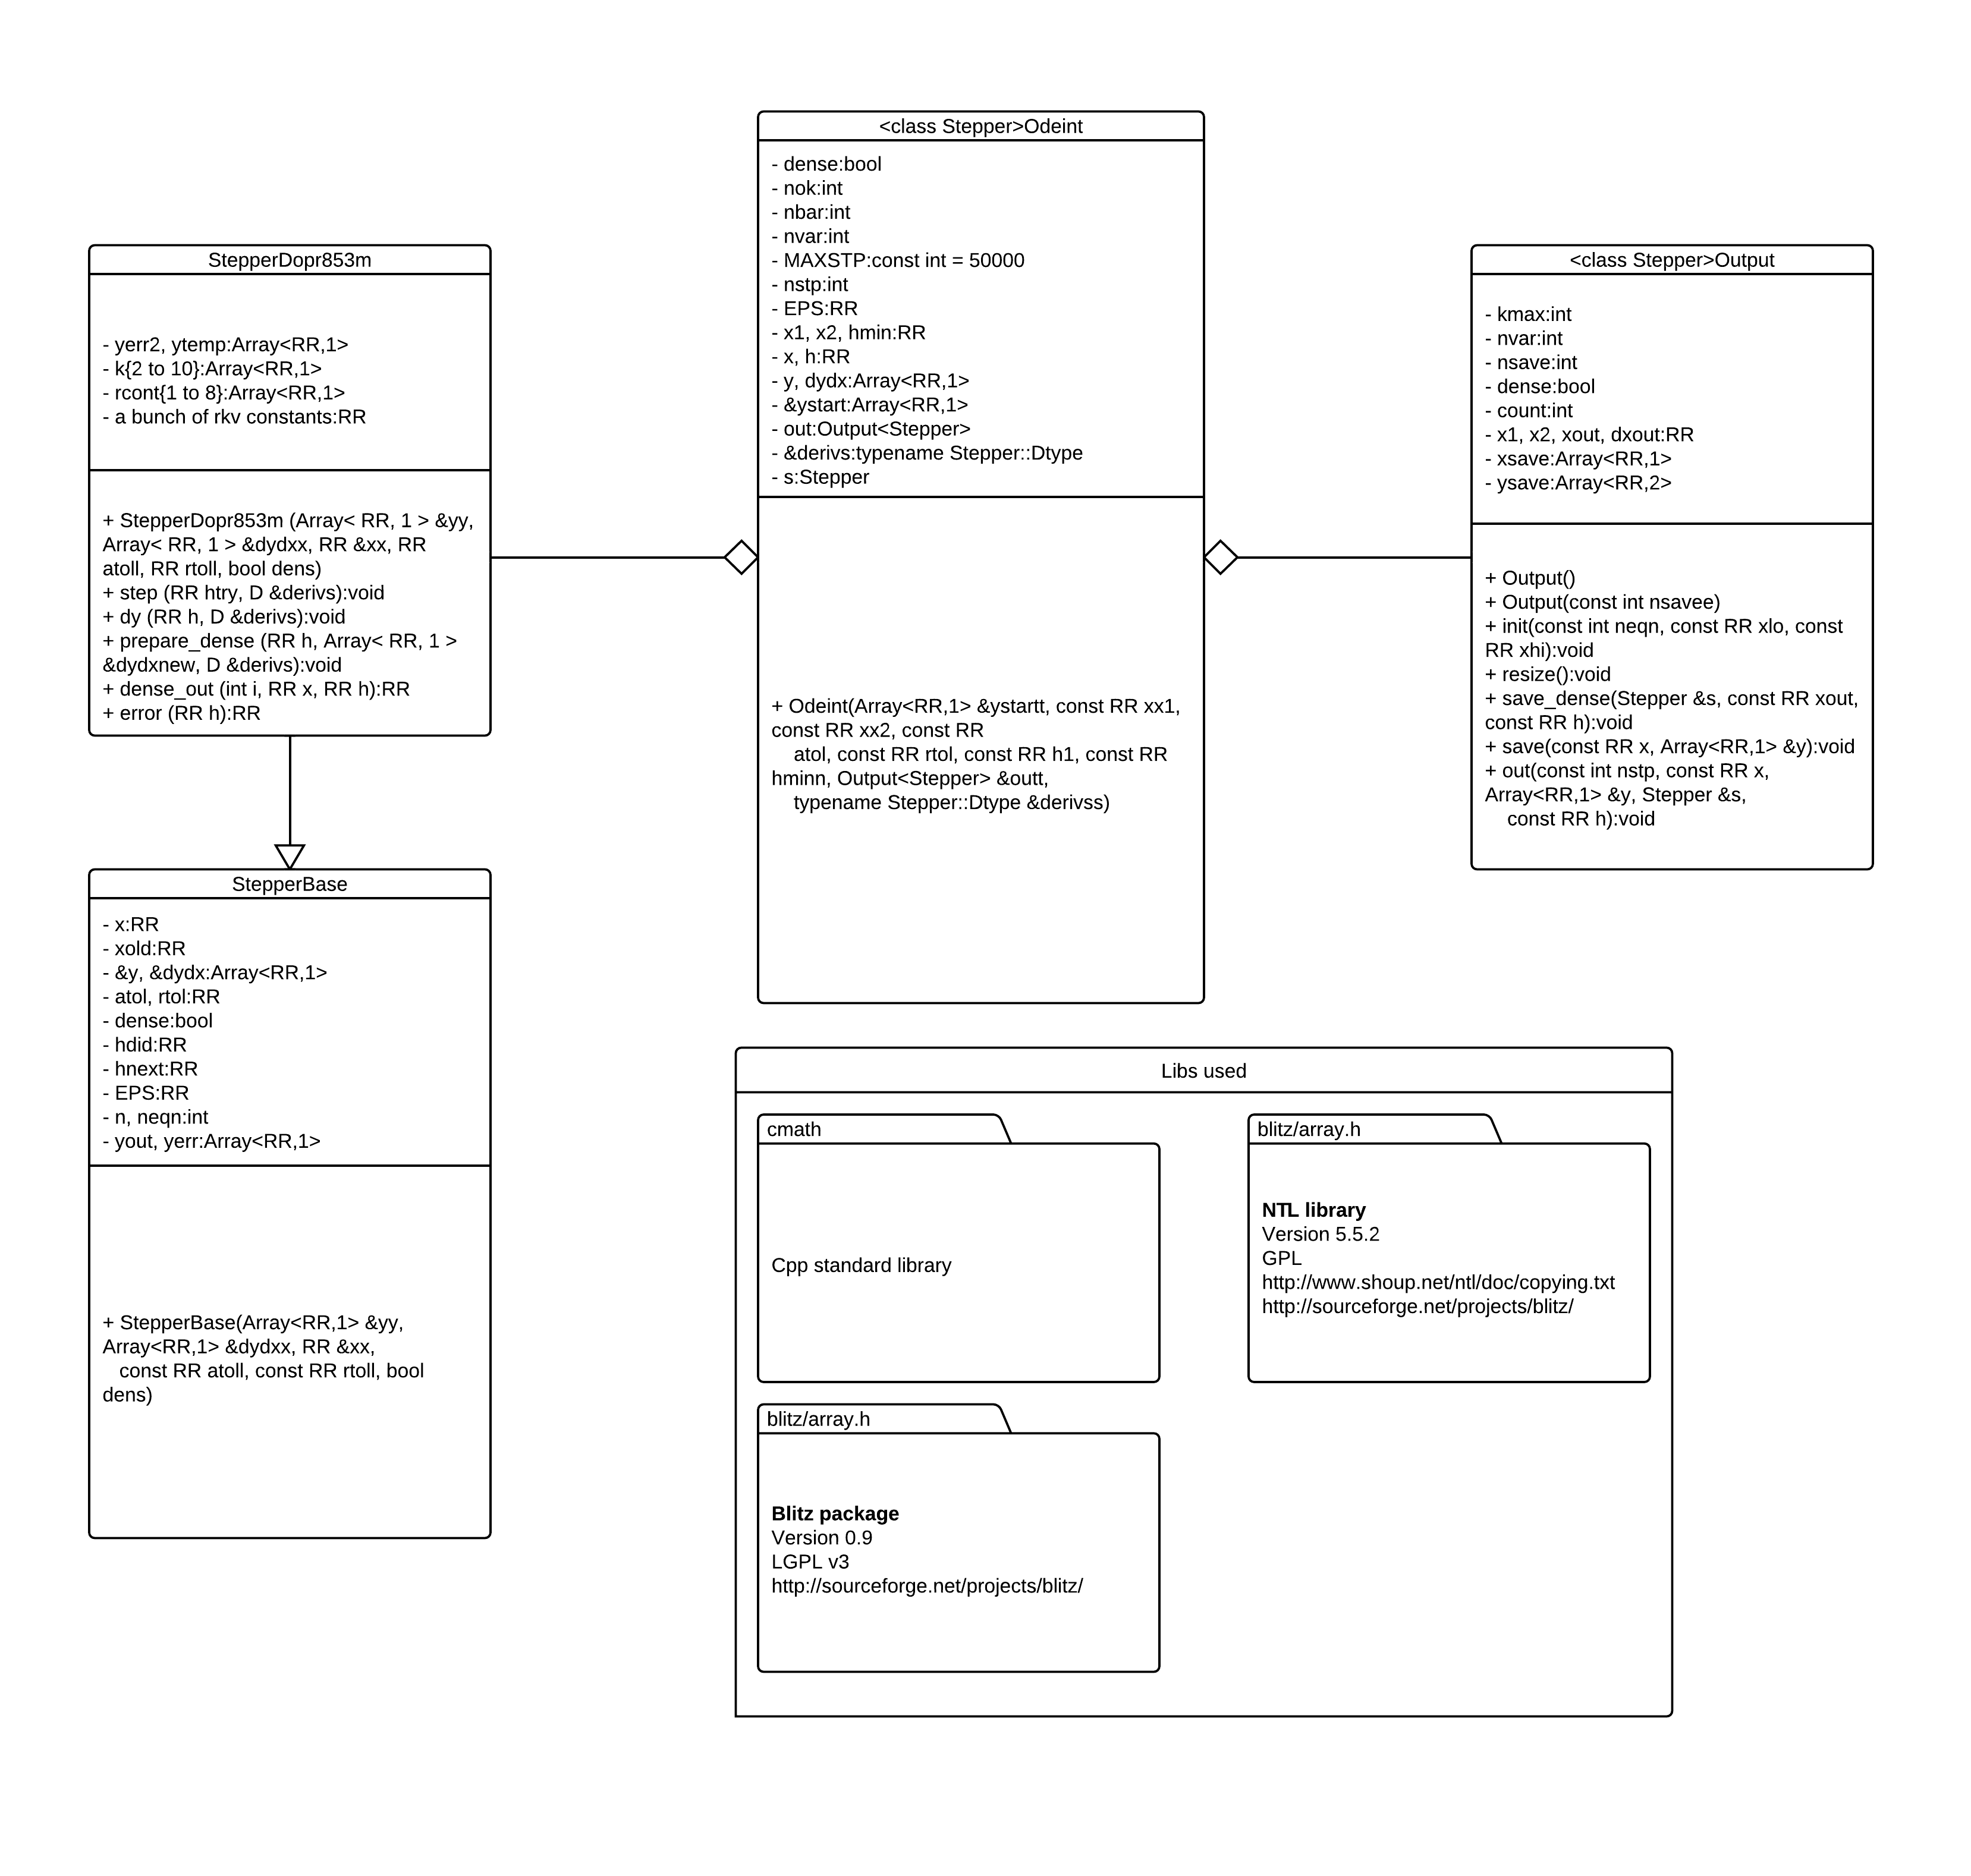
\includegraphics[width=4in,keepaspectratio=true]{figures/klassenidagramm.png}

\subsection*{StepperDopr853 - Dormand-Prince 853 method}
Entwicklungsschritte vom Prototypen zum fertigen L\"oser

Um Referenzdaten erzeugen zu k\"onnen und fr\"uhzeitig mathematische Fehler ausschlie\ss en zu k\"onnen haben wir uns f�r die Implementierung eines Prototypen entschieden.
Nach der ersten Implementierung eines rkv56 Verfahrens in Matlab entschieden wir uns, zu Gunsten einer h\"oheren Genauigkeit und Geschwindigkeit, weiter Implementierungen in Fortran95 zu programmieren.

Der fertige Fortran Prototyp, ebenfalls ein Runge-Kutta 56 mit adaptiver Schrittweitensteuerung, ben\"otigte f�r die L\"osung des TippeTop Problems\footnote[1]{$k=0.3, h_{min}=10^{-8}, h_{max}=10^{-6}, rtol=atol=10^{-4}, y0=(0.0, 0.0, 250.0, 0.0, 0.0, 0.1, 0.0, 0.0, 0.0, 0.0), T=[0,2.75], dG <10^{-6}, 3160922$ Einzelschritte.} \medskip

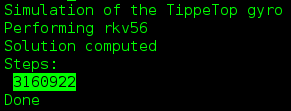
\includegraphics[width=2in,keepaspectratio=true]{figures/dopr0.png}

L\"osung des Prototypen f�r $\dot\psi$ in $rot/s$ \medskip

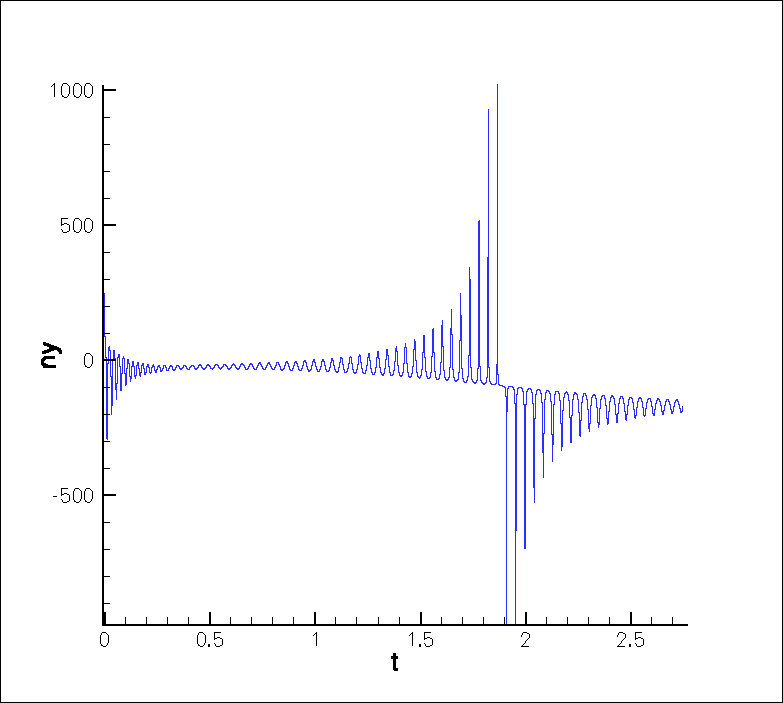
\includegraphics[width=4in,keepaspectratio=true]{figures/dopr1a.png}

Auf Grund der Erfahrung mit dem Prototypen entschieden wir uns f�r die Verwendung eines Dopr853 Verfahrens. Die erste Implementierung unter Verwendung des Datentyps double (auf ~15 Nachkommastellen genau) lieferte leider signifikant falsche Ergebnisse \medskip

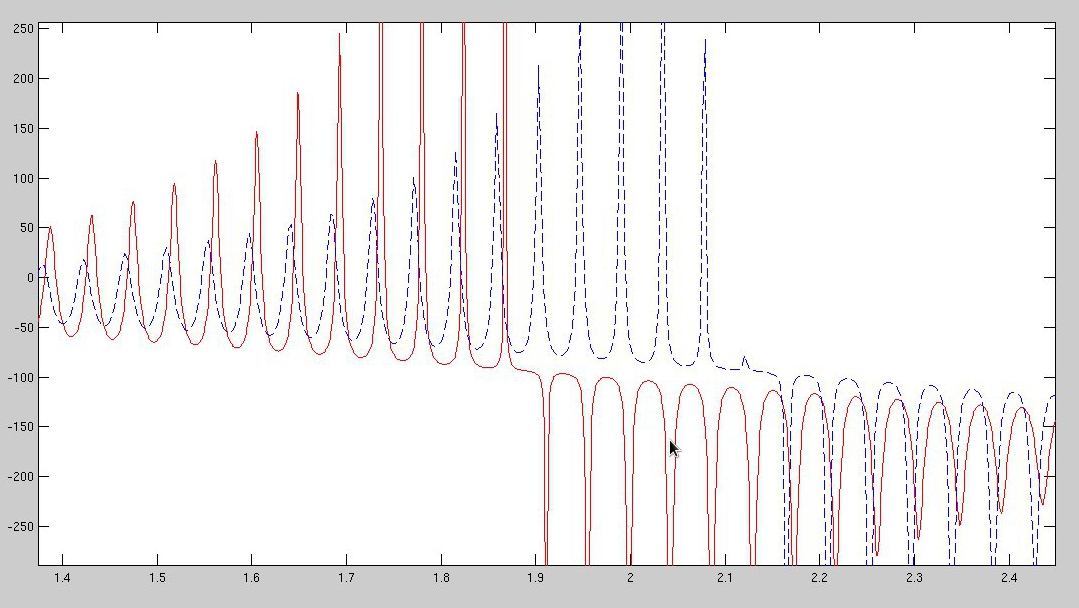
\includegraphics[width=4in,keepaspectratio=true]{figures/dopr1.png}

Die korrekte L\"osung der rkf56 Fortran95 Implementierung ist rot dargestellt, die falsche L\"osung des Dopr853$\_$double Algorithmus in blau. Es lag nahe das diese Unterschiede in der L\"osung auf Ungenauigkeiten in der Auswertung der steifen rechten Seite und den Berechnungen des Dopr853 Algorithmus zur\"uckzuf\"uhren waren. Wir entschieden uns also f�r die Verwendung eines genaueren Datentyps, und zwar NTL::RR aus der NTL library\footnote[2]{http://www.shoup.net/ntl/}

Unter verwendung des NTL::RR Datentyps kann der fertige L\"oser (Dopr853 in \textit{C++}) die L\"osung des Problems$^1$ in 852 Schritten berechnen. \medskip

L\"osung f�r $\dot\psi$(Drehgeschwindigkeit) mit Dopr853: \medskip

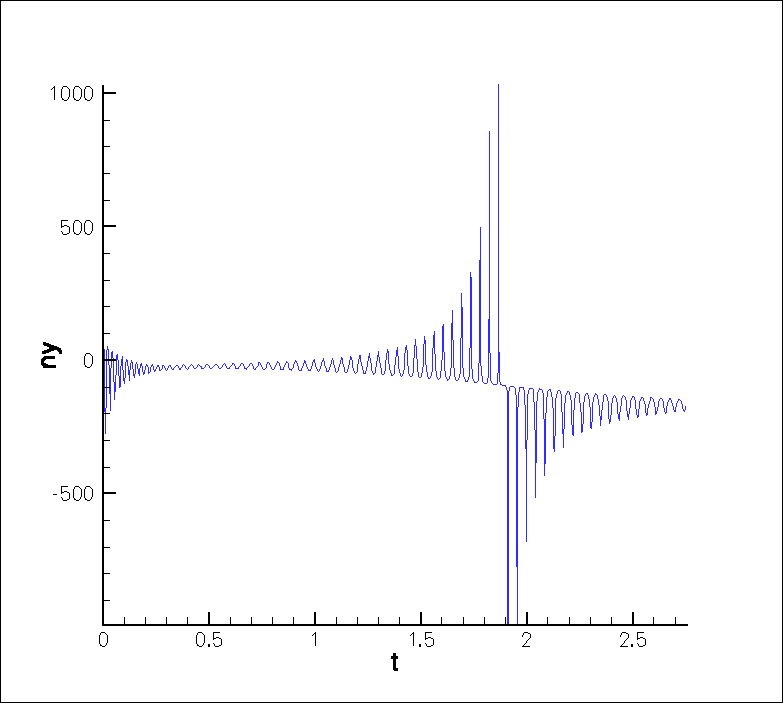
\includegraphics[width=4in,keepaspectratio=true]{figures/dopr2.png}

Der Dopr853 Algorithmus ist ein Algorithmus aus der Familie der Runge-Kutta Algorithmen der Ordnung 8.  F�r jeden Schritt werden 12 Auswertungen der rechten Seite des DGL ben\"otigt.
Der urspr\"ungliche Algorithmus nutzte eine Fehlersch\"atzung der Ordnung 6, was sich allerdings in einigen F\"allen als unzureichend herausstellte, da dieser Fehlersch\"atzer jeweils die letzte Auswertung nicht ber\"ucksichtigte. Hairer, N\"orsett und Wanner\footnote[3]{Hairer, E., N�rsett, S.P., and Wanner, G. 1993, Solving Ordinary Differential Equations I. Nonstiff 
Problems, 2nd ed. (New York: Springer). Fortran codes at 
http://www.unige.ch/~hairer/software.html } konstruierten Absch\"atzungen der f\"unften und dritten Ordnung, die auch den letzen Punkt ber\"ucksichtigen. Der Fehler kann also \"uber \\
$err = err_5 \frac{err_5}{\sqrt{(err_3)^2+0.01(err_5)^2}}$ \\
abgesch\"atzt werden. 

Die meiste Zeit \"uber gilt $err_5 << err_3$ und damit $err=O(h^8)$. \medskip

StepperDopr853 wurde als Mehrschrittverfahren mit fehlergesteuerter Schrittweitensteuerung implementiert, die neben dem gesch\"atzten Fehler auch noch die Erhaltungsgr\"o\ss e \\
$IR\dot\phi\sin^2\theta+I_3(R\cos\theta-a)(\dot\phi\cos\theta+\dot\psi) = const =: G$ \\
ber\"ucksichtigt. ($\Delta G$ pro Schritt $< 1E-6$ ).
Der L\"oser unterst\"utzt sowohl eine dichte Ausgabe \textit{dense output}, als auch die Ausgabe von n \"aquidistant verteilten Werten.\footnote[4]{Frei nach NumericalRecipes3rdEdition - Chapter 17.2.4 Dopr853 - An Eight-Order Method
Implementierung nach Numerical Recipes Software 2007, "Routine Implementing an Eighth-order Runge-Kutta Method,"
Numerical Recipes Webnote No. 20, at http://www.nr.com/webnotes?20}

\newpage
\section{Graphical User Interface}
\label{sec:3.3}
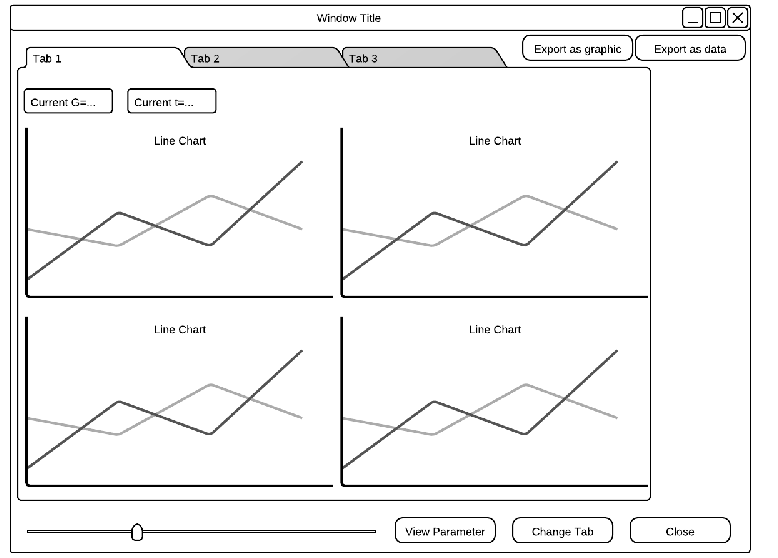
\includegraphics[width=4in,keepaspectratio=true]{figures/GUIDisplayForm.png}

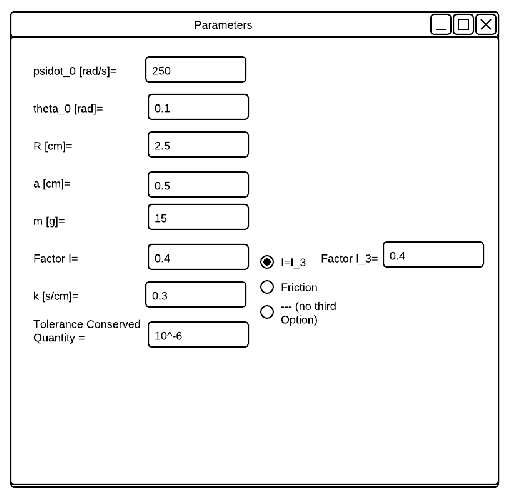
\includegraphics[width=4in,keepaspectratio=true]{figures/GUIParameterInputForm.png}

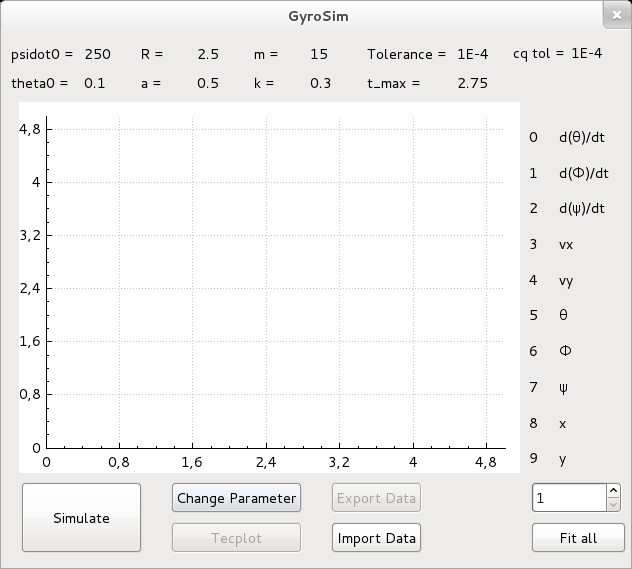
\includegraphics[width=4in,keepaspectratio=true]{figures/mainwindow_clean.png}

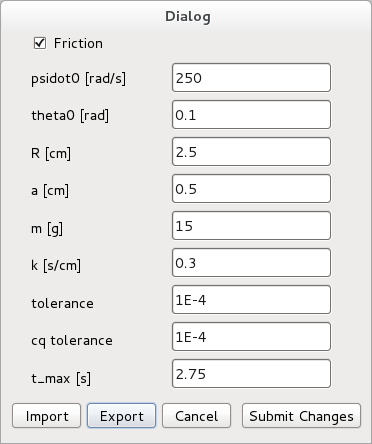
\includegraphics[width=4in,keepaspectratio=true]{figures/change_parameter_default.png}
\section{Use-Case-Diagramm}
\label{sec:3.4}
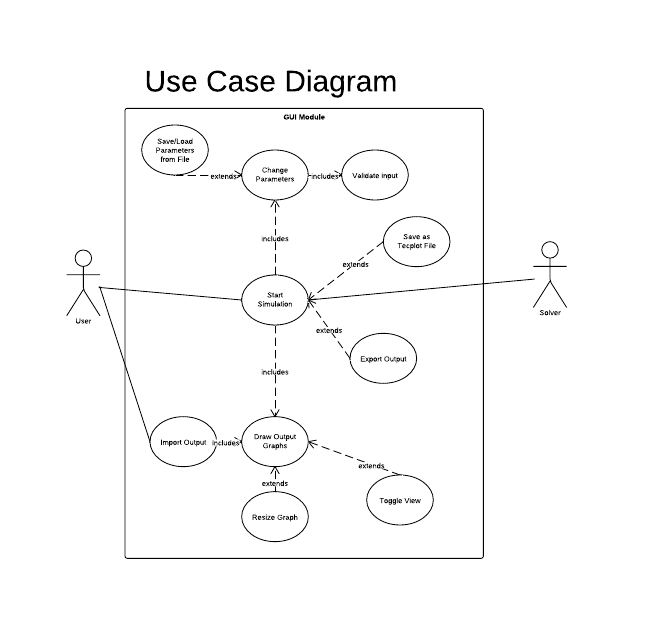
\includegraphics[width=6in,keepaspectratio=true]{figures/UseCaseTippeTop.png}

